\documentclass[a4paper]{article}
\pagestyle{headings}
\usepackage[utf8x]{inputenc}
% \usepackage{polski}
\usepackage{color}
\usepackage{transparent}
\usepackage{graphicx}
\graphicspath{{images/}}
\usepackage{listings}
\usepackage{courier}
\usepackage{amsmath}
\usepackage{syntax}
\usepackage{url}



\usepackage{wrapfig}

\grammarindent8em
\newtheorem{defi}{Definition}[section]

\definecolor{javared}{rgb}{0.6,0,0} % for strings
\definecolor{javagreen}{rgb}{0.25,0.5,0.35} % comments
\definecolor{javapurple}{rgb}{0.5,0,0.35} % keywords
\definecolor{javadocblue}{rgb}{0.25,0.35,0.75} % javadoc

 \lstloadlanguages{
         Java
 }
 \lstset{language=Java,
         basicstyle=\footnotesize\ttfamily, % Standardschrift
         %numbers=left,               % Ort der Zeilennummern
         numberstyle=\tiny\color{black},          % Stil der Zeilennummern
         stepnumber=1,               % Abstand zwischen den Zeilennummern
         numbersep=5pt,              % Abstand der Nummern zum Text
         tabsize=1,                  % Groesse von Tabs
% 	inputencoding=utf8, extendchars=\true
         extendedchars=true,         %
         breaklines=true,            % Zeilen werden Umgebrochen
keywordstyle=\color{javapurple}\bfseries,
stringstyle=\color{javared},
commentstyle=\color{javagreen},
morecomment=[s][\color{javadocblue}]{/**}{*/},
    		frame=b,         
 %        keywordstyle=[1]\textbf,    % Stil der Keywords
 %        keywordstyle=[2]\textbf,    %
 %        keywordstyle=[3]\textbf,    %
 %        keywordstyle=[4]\textbf,   \sqrt{\sqrt{}} %
         stringstyle=\color{white}\ttfamily, % Farbe der String
         showspaces=false,           % Leerzeichen anzeigen ?
         showtabs=false,             % Tabs anzeigen ?
         xleftmargin=17pt,
         framexleftmargin=17pt,
         framexrightmargin=5pt,
         framexbottommargin=4pt,
         %backgroundcolor=\color{lightgray},
         showstringspaces=false      % Leerzeichen in Strings anzeigen ?        
 }
    %\DeclareCaptionFont{blue}{\color{blue}} 

  %\captionsetup[lstlisting]{singlelinecheck=false, labelfont={blue}, textfont={blue}}
  \usepackage{caption}
\DeclareCaptionFont{white}{\color{white}}
\DeclareCaptionFormat{listing}{\colorbox[cmyk]{0.43, 0.35, 0.35,0.01}{\parbox{\textwidth}{\hspace{15pt}#1#2#3}}}
\captionsetup[lstlisting]{format=listing,labelfont=white,textfont=white, singlelinecheck=false, margin=0pt, font={bf,footnotesize}}



\newcommand{\jls}{The Java\texttrademark Language Specification}
\newenvironment{zalozenie}{\textbf{Assumptions}:\begin{enumerate}}{\end{enumerate}}


%opening
\title{Service Architecture Model \\ Draft 0.2}
\author{Paweł Cesar Sanjuan Szklarz \\ \texttt{paweld2@gmail.com}}
\date{\today}






\begin{document}
\maketitle

\begin{abstract}
Service Architecture Model (SAM) is a mathematical model for definition of service oriented architectures. SAM Architecture products are defined using code and precisely defined relations. Validation of architecture is based on a compilation process. It is also possible to automatically verify implementations compliance with service specifications. A development and verification process for service implementation is also defined. A key idea behind SAM is the use of a canonical execution protocol, intuitively related to ``methods execution recording''.
\end{abstract}

\null\vfill
\noindent
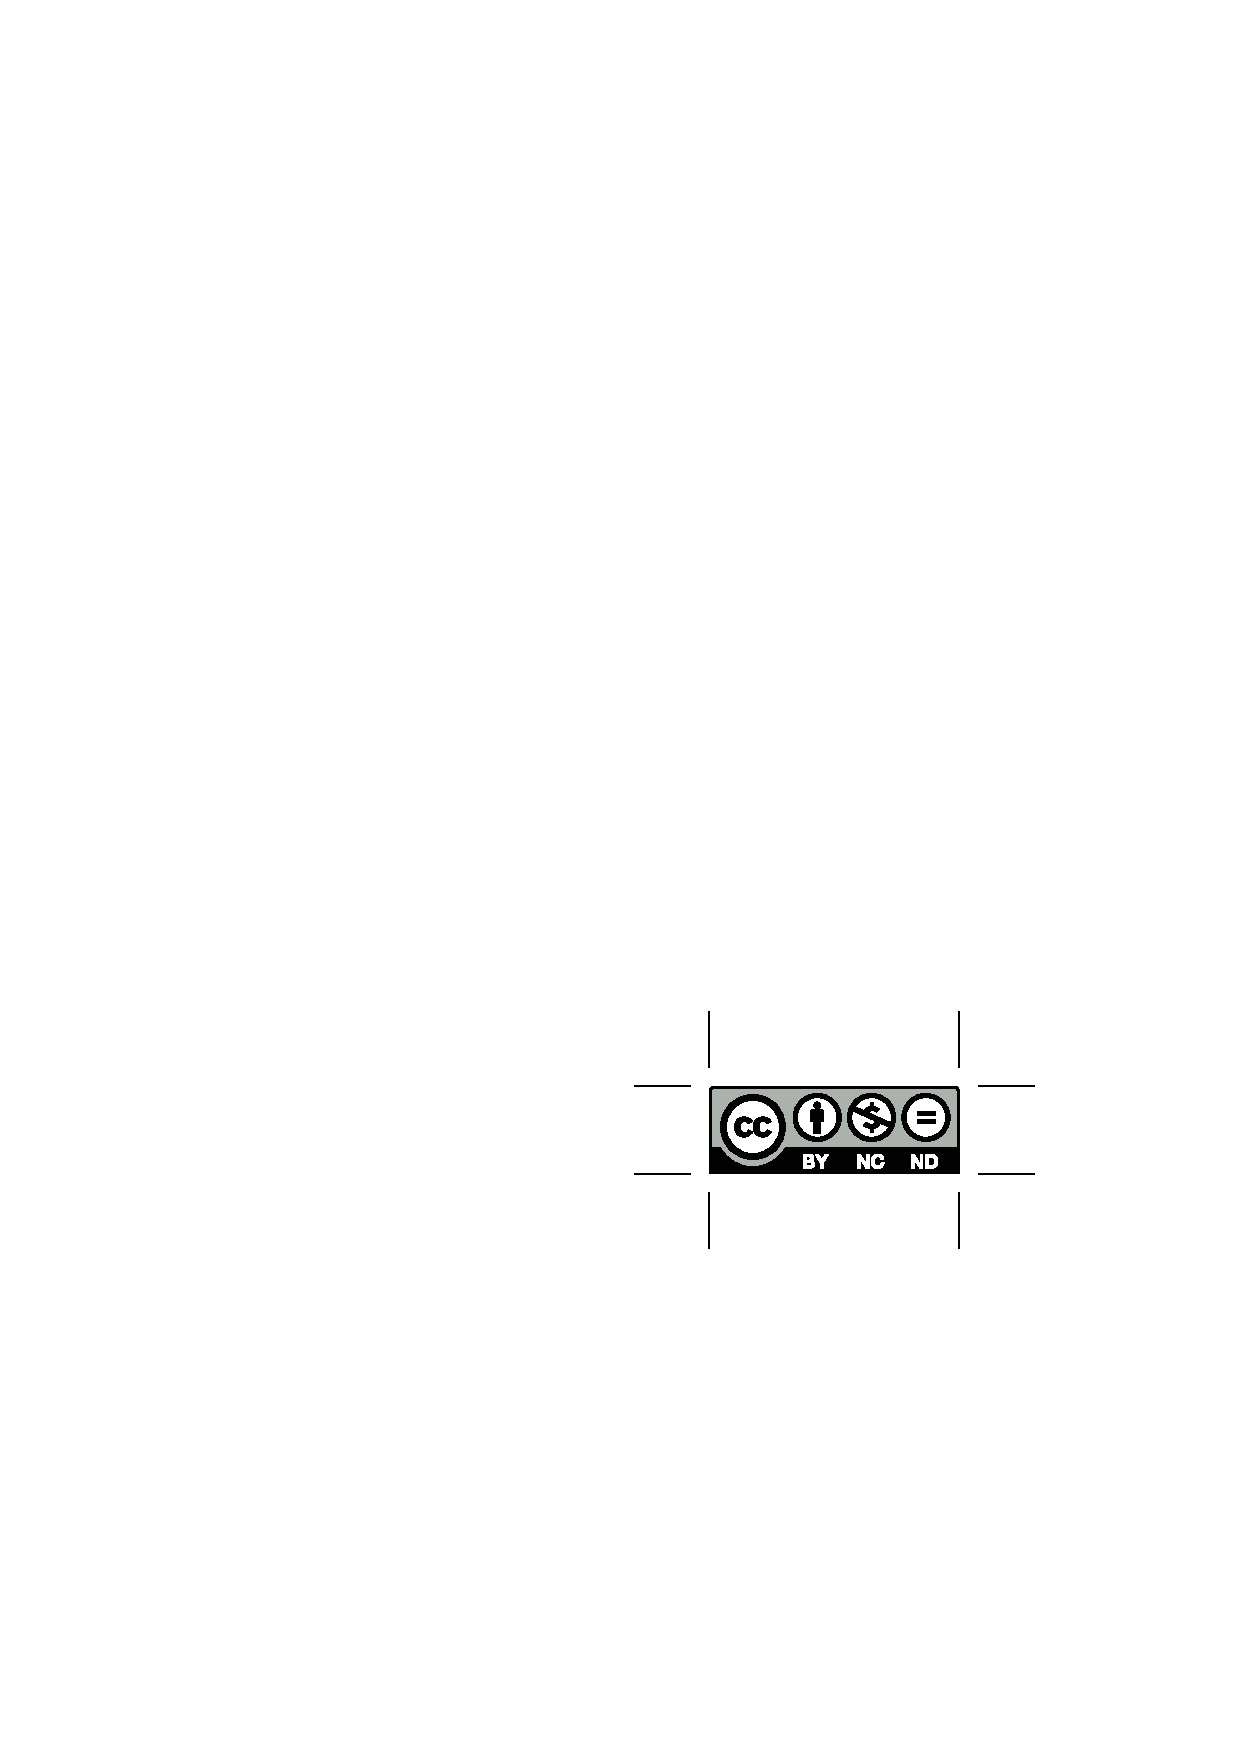
\includegraphics[scale=0.5]{by-nc-nd}
This work is licensed under a Creative Commons Attribution-NonCommercial-NoDerivs 3.0 Unported License.

\noindent\line(1,0){340}

\noindent
Copyright \textcopyright 2011 Paweł Cesar Sanjuan Szklarz

\newpage
% \input{title}

\tableofcontents 
\null\vfill\noindent\newpage
\listoffigures
\null\vfill\noindent\newpage
\section{Introduction}

% TODO Zrobic wstep do wstepu


The documentation is ordered as follows. This sections contains a intuitive overview of Service Architecture Model. Section \ref{sec:samModel} present a precise definition of presented concepts. Abstract Domain Dependency Model defined on section \ref{sec:ioc} is necessary to define service injection. Section \ref{sec:SEE} present a execution model for services of a SAM Architecture.

\subsection{Architecture Overview}

A SAM \textbf{Architecture} defines a \textbf{Service Taxonomy}. Service Taxonomy is a set of separate \textbf{Categories} grouping \textbf{Service Specifications}.

\begin{figure}[h!]
 \centering
 \includegraphics[width=1\textwidth]{taxonomy}
 \caption{Service Taxonomy example}
 \label{fig:taxonomy}
\end{figure}

Figure \ref{fig:taxonomy} shows a service taxonomy consisting of five categories. Each category has different Service Specifications indicated by dots.

% TODO referencja do javy -> zmienic na opis method jako R name(args)
A \textbf{Service Specification} is a set of \textbf{Interfaces}. A Interface intuitively should be treated as a normal Java interface. No class members are allowed on Interfaces. Service Specifications are disjoint.

For one Service Specification it is possible to have many different Service Implementations. A \textbf{Service Implementation} or Implementation is a \textbf{Binding Provider} (see section \ref{sec:ioc}) and all necessary classes to instantiate the Service Specification Interfaces. For simplicity, one can assume that it is a set of classes implementing the Service Specification Interfaces. See \ref{sec:ServiceImplementation} for more details about Service Implementations.

Implementations are executed on a \textbf{Service Execution Environment}. One Implementation executed is called a \textbf{Service Instance} or Instance for short, and it has a unique \textbf{Instance Identificator} (IID). It is possible to execute many Service Instance of the same Service Specification simultaneously. Each Service Instance can be a instantiation of a different Implementation. See section \ref{sec:intSEE} for a overview of Service Execution Environment and section \ref{sec:SEE} for reference information.

To use external services, the Implementation developer must introduce to the code references to interfaces belonging to some external services. \textbf{Dependency Injection Model} is used to inject references to  Service Instances of appropriate type. The choose of  external Service Instance is made completely on the Service Execution Environment as a configuration aspect. The exact definition of Dependency Injection Model is given in section \ref{sec:ioc}.

SAM imposes constraints on the external services used in Implementations defined be a \textbf{Category Accessibility Relation}:  category $C_2$ is accessible to category $C_1$ if we allow injection of interface of services from category $C_2$ in the implementation of services of $C_1$. As an example, assume that category accessibility relation for architecture given in figure \ref{fig:taxonomy} is as follow:
\begin{eqnarray}
\text{User Services} &\hookleftarrow & \text{Core Services} \nonumber \\
\text{Core Services} &\hookleftarrow& \text{Core Services} \nonumber \\
\text{Core Services} &\hookleftarrow& \text{Infrastructure Services} \nonumber \\
\text{Core Services} &\hookleftarrow& \text{Management Services} \nonumber \\
\text{Core Services} &\hookleftarrow& \text{Information Services} \nonumber 
\end{eqnarray}

This mean that a Service Implementations of Service Specification belonging to Category ``User Services'' can inject only references to Service Instances belonging Category ``Core Service''.

\subsection{Service Specification}

We present on more detailed overview of Service Specification definition and some concrete examples.

% TODO cambiar el nombre del service
Lets see the definition of ``UserData'' Service Specification belonging to Category ``User Service''. It is defined be two interface's as shown on listing \ref{UserServiceSimple},\ref{UserServiceComplex}.

\lstinputlisting[label=UserServiceSimple,caption=Service Specification Interface API - UserData]{../srcAPI/eu/pmsoft/sam/service/user/UserDataSimpleAPI.java}

Method \lstinline|simpleMethod| is just a simple example without arguments and return type \lstinline|boolean|. Method \lstinline|complexInteractionAPI| is more interesting, it has a simple type argument and returns a reference to interface \lstinline|UserDataComplexAPI| defined below. On SAM Interface methods signature it is allowed to use only primitive types and interface types declared on the architecture.

A important relation between Interfaces is the \textbf{Signature Relation} resulting from the types used on methods signatures. As a examples we say that Interface \lstinline|UserDataSimpleAPI| uses Type related to \lstinline|UserDataComplexAPI| because it appears as a return type of method \lstinline|complexInteractionAPI|. Please note that Signature Relation is defined between Interfaces and Types resulting from Interfaces.

\lstinputlisting[label=UserServiceComplex,caption=Service Specification Interface API - UserData]{../srcAPI/eu/pmsoft/sam/service/user/UserDataComplexAPI.java}

Interface \lstinline|UserDataComplexAPI| is very similar to previous one. It defines three methods with some parameters and result types. Note that there are two new interfaces \lstinline|DomainData| and \lstinline|DomainTypeExample| not belonging to the Service Specification. A set of interfaces used on a Service Specification is called a \textbf{Domain Specification}. It is required for Domain Specifications to be mutually disjoint.

% , shown on listing \ref{DomainData},\ref{DomainTypeExample}
% \lstinputlisting[label=DomainData,caption=DomainData Interface]{../srcAPI/eu/pmsoft/sam/ds/DomainData.java}
% \lstinputlisting[label=DomainTypeExample,caption=DomainTypeExample Interface]{../srcAPI/eu/pmsoft/sam/ds/DomainTypeExample.java}

Signature Relation implies a \textbf{Domain Dependency Relation} between Domain Specifications: If a type derived from Domain Specification $d_2$ is used on some method signature of a Interface from Domain Specification $d_1$, then we say that $d_1$ depends on $d_2$.

We treat Service Specification as a Domain Specification, but do not allow to use Types from Service Specifications on other Domain Specifications. We also require that the Domain Dependency Relation be acyclic. A possible graph related to a Domain Dependency Relation is shown on figure \ref{fig:service}.

\begin{figure}[ht!]
 \centering
 \includegraphics[width=1\textwidth]{serviceSpec}
 \caption{Domain Dependency Relation example}
 \label{fig:service}
\end{figure}

A Domain Specification without dependencies is called a Simple Domain Specification. If it has dependencies, then is called Model Domain Specification. As mentioned earlier, a Service Specification can't be used as a dependency.



Lets define a Service Specification ``CoreServiceExample'' containing interface \ref{CoreServiceExample} to be used in the following examples.

\lstinputlisting[label=CoreServiceExample,caption=CoreServiceExample Service Specification]{../srcAPI/eu/pmsoft/sam/service/core/CoreServiceExample.java}


\subsection{Service Implementation and Service Instance Injection}
\label{sec:ServiceImplementation}

A simple implementation ONE of Service Specification ``CoreServiceExample'' is class \lstinline|ImplementationCoreServiceExampleOne| implementing interface \lstinline|CoreServiceExample|, see listing \ref{ImplementationCoreServiceExampleOne}.

\lstinputlisting[label=ImplementationCoreServiceExampleOne,caption=Implementation ONE of ``CoreServiceExample'']{../srcAPI/eu/pmsoft/sam/impl/core/ImplementationCoreServiceExampleOne.java}

Note fields of Type \lstinline|CoreServiceExample|. These are examples of \textbf{Injection Points}, places where it is possible to receive injections, it is references to external Service Instance. Field \lstinline|public CoreServiceExample serviceInjectionPointWithBindingAnnotation;| has also a Binding Annotation. \textbf{Binding Annotations} instruct the Service Execution Environment on how to interconnect Service Instances. Each Injection Point has associated a \textbf{Key} defined as a pair Type-Binding Annotation. Binding Annotation may be empty.

A Implementation TWO of ``CoreServiceExample'' is created with classes \lstinline|ImplCoreTwo|,\lstinline|ImplCoreTwoBinding| and a non trivial Binding Provider following scheme:
\begin{eqnarray}
\text{CoreServiceExample}\times 0 &\longmapsto& \text{ImplCoreTwo} \nonumber \\
\text{CoreServiceExample}\times\text{@BindingAnnotationExample} &\longmapsto& \text{ImplCoreTwoBinding} \nonumber 
\end{eqnarray}
Implementation TWO provides a different class implementing \lstinline|CoreServiceExample| according to used Key.

Assume that on the Service Execution Environment are created two Instances of Service Specification ``CoreServiceExample'' using previously presented Implementations ONE and TWO, with IID ``01'' and ``02'' respectively.

Service Execution Environment could be configured to inject Instance ``02'' to Instance ``01'' as shown in figure \ref{fig:instanceinjection01}.

\begin{figure}[h!]
 \centering
 \includegraphics[width=1\textwidth]{instanceInjection01}
 \caption{Service Instance injection}
 \label{fig:instanceinjection01}
\end{figure}

Other possible scenario is to inject Instance ``01'' on Instance ``01'' as shown on figure \ref{fig:instanceinjection02}. Implementation ONE don't define any binding for key $\text{CoreServiceExample}\times \text{@BindingAnnotationExample}$, so the simplest key $\text{CoreServiceExample}\times 0$ is used because it also match the annotated Injection Point.

\begin{figure}[h!]
 \centering
 \includegraphics[width=1\textwidth]{instanceInjection02}
 \caption{Self-Reference injection}
 \label{fig:instanceinjection02}
\end{figure}

For details on Dependency Injection Model and Injection Process see section \ref{sec:ioc}.

\subsection{Service interaction and Canonical Execution Protocol}
\label{sec:intCallProtocol}

Existing service interaction methods and technologies are based on a function execution abstraction, a service is understood as a external set of functions available through remote calls. This approach leads to the following logical scheme during architecture and software development:
\begin{itemize}
 \item Prepare service request data
 \item Execution: Send service request, wait for response
 \item Interpret response
\end{itemize}
Such a pattern is associated with high costs related to calls on external service. This leads to creation of increasingly complex data structures to define the parameters and results of service methods, or ``external functions''.

SAM introduce a completely new approach to service calls and service interaction. To illustrate this,  lets use a Implementation of ``UserData'' Service Specification that contain class \lstinline|ImplementationOneSimple| shown on listing \ref{ImplementationOneSimple}.
% ,\ref{ImplementationOneComplex}.
% and \lstinline|ImplementationOneComplex|

\lstinputlisting[label=ImplementationOneSimple,caption=Class of UserData Implementation]{../srcAPI/eu/pmsoft/sam/impl/user/one/ImplementationOneSimple.java}

Method \lstinline|public boolean simpleMethod()| is implemented using external service ``CoreServiceExample''. Note that executing this method may require a large number of calls to interface \lstinline|CoreServiceExample|, but how many external requests are needed? only one!. See listing \ref{CoreServiceExample} for the definition of interface \lstinline|CoreServiceExample| and note that only the \lstinline|isProcessStatusOk| method has a return type different that \lstinline|void|. SAM define a \textbf{Canonical Execution Protocol} to serialize calls to Service Specification Interfaces. Execution of method \lstinline|public boolean simpleMethod()| serialized with the canonical protocol produce a service request containing:
\begin{verbatim}
i_0.resetProcess()|i_0.putData(i_1)|...
...i_0.putData(i_n)|i_0.isProcessStatusOk()r_0|
PAYLOAD
i_0=KEY<CoreServiceExample X 0>
i_1="IntegerSerialization"
...
i_n="IntegerSerialization"
r_0=Type<boolean>
\end{verbatim}

This is the exact information necessary for a external Service Instance implementing ``CoreServiceExample'' to repeat calls to interface \lstinline|CoreServiceExample| and return the final result.



Generally, an external call is required when the return type of a Interface method is a class type. In the case that a return type is a interface type, it is possible to continue ``recording'' executions to that interface without any external request. See method \lstinline|changeUserName| on listing \ref{CanonicalWithInterface} and resulting canonical service request.

\lstinputlisting[label=CanonicalWithInterface,caption=Calls to external service with nested interface executions]{../srcAPI/eu/pmsoft/sam/examples/ServiceCode.java}

\begin{verbatim}
i_0.sendData(i_1)r_0|r_0.sendMoreData(i_2)r_1|
PAYLOAD
i_0=KEY<ExternalServiceInterface X @BindingAnnotationExample>
r_0=InterfaceType<NestedExternalInterface>
i_1="IntegerSerialization"
i_2="StringSerialization"
r_1=Type<Boolean>
\end{verbatim}
In this case also, only one external request is necessary to realize service interaction.

The reason for which Domain Specifications consist only of interfaces is to maximize the possible sequences of calls without exchange of requests between Service Instances.

\subsection{Service Implementation development}
\label{sec:intImpleDEVEL}



A Service Implementation that don't inject any external Service is called a \textbf{Prototype Implementation} or Prototype. During development of any Service Implementation, it is very convenient to have Prototypes for each used Service Specification. If a Prototype implementation of each used Service Specification is available, then a local execution environment can be easily created.


Having Prototypes injected it is possible to execute internal tests. A SAM Architecture can additionally provide predefined tests for a given Service Specification called Test Specification. \textbf{Test Specification} is a set of test classes containing injection points only for one given Service Specification. Note that Test Specifications can be developed independently of any Service Implementations.The use of Canonical Execution Protocol for service interaction makes possible to create Test Specification on base of previously recorded services interaction. In case that a complex bug is found on some Implementation, a test case could be recorded and then executed on all existing Implementations.

Using Prototypes and Test Specifications on development process leads to Service implementations with defined injection as in figure \ref{fig:serviceImplementation}.

\begin{figure}
 \centering
 \includegraphics[width=1\textwidth]{serviceImplementation}
 \caption{Service Implementation injection for development}
 \label{fig:serviceImplementation}
\end{figure}

\newpage
\subsection{Service Execution Environment}
\label{sec:intSEE}

Execution of a Service Implementation to create Service Instances is done by injecting dependencies for some existing Service Instance. Injection Process defined on section \ref{sec:iocIP} support such execution process, allowing also the creation of cyclic injections between Service Instance. Each Service Instance gets a unique Instance ID (IID).

\textbf{Injection Configuration} defining Service Instance injection is a mapping
\begin{eqnarray}\label{sseconfig}
config: IID \times Service Specification \longrightarrow IID \nonumber
\end{eqnarray}
maintained by a \textbf{Service Execution Environment}.

Note that Service Implementations don't have any control over the injection process, they don't even have knowledge of IID of injected Service Instances. All the control over Service Instance injection is transferred to the Service Execution Environment.

Given two Injection Configurations, it is possible to merge then in a new mapping. This ensure Service Execution Environment scalability.

Two Service Execution Environments not trusting each other, can share limited information about running Services Instances and enable service interaction under the supervision of special security policies.






\null\vfill\noindent\newpage
\newpage
\section{Service Architecture Model}
\label{sec:samModel}
This section define precisely all the Service Architecture Model concepts and assumptions.

To remark the use of SAM concepts on the text Start Case is used for concept names.

Defined sets and relations are related to one Architecture defined using Service Architecture Model.

\subsection{Types and Interface}

A object oriented approach is taken to define Types and Interfaces.

\begin{defi}[Basic Type]
  A predefined set of primitive types.
\end{defi}

A concrete list of accessible Basic Types is related to a given implementation of SAM. Bindings to specific programming languages may define mappings between provided Basic Types on SAM implementation and language types.

\begin{defi}[Type]
  Basic Type and Interface Types uniquely defined by a Interface.
\end{defi}

\begin{defi}[Interface]
  Interface is a set of methods. Method signature is defined by a
\begin{itemize}
 \item method Name
 \item return Type
 \item list of arguments (list of Types)
\end{itemize}
\end{defi}

An Interface should be uniquely identified by a name.

% \begin{zalozenie}
%  \item Architecture Interfaces don't have class members.
% \end{zalozenie}


The set of Interfaces is denoted by $\mathcal{I}$. The set of Types is denoted by $\mathcal{T}$. The set of Basic Types is denoted by $\mathcal{B}\subset\mathcal{T}$.

The mapping between Interface and corresponding Interface Type is denoted by function $t$
\begin{eqnarray}
t:\mathcal{I}\rightarrow\mathcal{T}
\end{eqnarray}
and implies also a function $\tilde{t}$ between Interfaces sets to Types sets defined as:
\begin{eqnarray}
\tilde{t}:2^\mathcal{I}\rightarrow 2^\mathcal{T} \quad
 \tilde{t}(\{i_1,\dots,i_\alpha\}) := \{t(i_1),\dots,t(i_\alpha) \}
\end{eqnarray}

\begin{defi}[Signature Relation]
  Interface `$i$' is signature related to Type `$t$' if a method signature of `$i$' contains `$t$'. This relation is denoted by set `$\mathring{s}$':
\begin{eqnarray}
\mathring{s}\subset \mathcal{I}\times \mathcal{T}
\end{eqnarray}
\end{defi}

\begin{defi}[Signature Maps]
The Signature Map is the function $s$
\begin{eqnarray}
&s:\mathcal{I}\rightarrow 2^\mathcal{T}&
\end{eqnarray}
given by the statement:
\begin{eqnarray}
&(i,t) \in \mathring{s} \Rightarrow t\in s(i) &\nonumber
\end{eqnarray}

A set version of the Signature Map is defined by function $\tilde{s}$
\begin{eqnarray}
&\tilde{s}:2^\mathcal{I}\rightarrow 2^\mathcal{T}& 
\end{eqnarray}
defined as 
\begin{eqnarray}
&\tilde{s}(\{i_1,\dots,i_\alpha\}) := s(i_1) \cup \dots \cup s(i_\alpha) &
\end{eqnarray}

\end{defi}

\begin{zalozenie}
 \item For a given Architecture, Signature methods of Interfaces use only Basic Types or Types defined by Interfaces belonging to the given Architecture.
\end{zalozenie}

\subsection{Domain Specification Model}

\begin{defi}[Domain Specification]
  A named set of Interfaces.
\end{defi}

\begin{zalozenie}
 \item Domain Specifications on Architecture are mutually disjoint.
\end{zalozenie}

% The set of Interfaces is denoted by $\mathcal{I}$. The set of Types related to $\mathcal{I}$ is denoted by $\mathcal{T}$. The set of Basic Types is denoted by $\mathcal{B}\subset\mathcal{T}$.

The set of Domain Specifications is denoted by $\mathcal{D}$. Because for $d \in \mathcal{D}$ we have $d \subset 2^\mathcal{I}$, function $\tilde{t}$ and $\tilde{s}$ are well defined on $\mathcal{D}$.

\begin{defi}[Domain Dependency Relation]
  Domain Specification $d_1$ \textbf{depends on} Domain Specification $d_2$ $[(d_1,d_2)\in \delta]$, if a Type related to a Interface belonging to $d_2$ is used on a method signature of a Interface belonging to $d_1$
\begin{eqnarray}
 &\delta \subset \mathcal{D} \times \mathcal{D} &\\
&\tilde{t}(d_2) \cap \tilde{s}(d_1) \neq \emptyset  \Rightarrow (d_1,d_2) \in \delta  &\nonumber
\end{eqnarray}
\end{defi}

\begin{zalozenie}
 \item Domain Dependency Relation $\delta$ is acyclic.
\end{zalozenie}

Simple Domain Specification is a Domain Interfaces that use in methods signature only Basic Types and own Types, precisely:
\begin{defi}[Simple Domain Specification]
  Domain Specification $d$ such that
\begin{eqnarray}
\tilde{s}(d) \subset \mathcal{B} \cup \tilde{t}(d)
\end{eqnarray}
\end{defi}

Definition implies that Simple Domain Specification don't depend on any Domain Specification.

\begin{defi}[Model Domain Specification]
  Domain Specification that depends on other Domain Specification.
\end{defi}

\subsection{Service Specification}

\begin{defi}[Service Specification]
  A Model Domain Specification.
\end{defi}

\begin{zalozenie}
 \item Services are not used as Domain Dependencies: if $s$ is a Service Specification, then
\begin{eqnarray}
 \forall d \in \mathcal{D} \quad  (d,s) \notin \delta
\end{eqnarray}
\end{zalozenie}

The set of Service Specification is denoted by $\mathcal{S}$, we have $\mathcal{S} \subset \mathcal{D}$.

\subsection{Taxonomy and Category}

\begin{defi}[Taxonomy]
  Equivalence relation of Services Specifications
\begin{eqnarray}
 \tau \subset \mathcal{S}  \times \mathcal{S} 
\end{eqnarray}
\end{defi}

\begin{defi}[Category]
  Equivalence class of Taxonomy.
\end{defi}

The set of Categories is denoted by $\Gamma$. Taxonomy projection is denoted by
\begin{eqnarray}
cat: \mathcal{S} \rightarrow \Gamma
\end{eqnarray}

\subsection{Service Implementation}

Service Implementation definition is based on Dependency Injection Model presented on section \ref{sec:ioc}.

\begin{defi}[Architecture Annotations]
  A set of Binding Annotations.
\end{defi}

\begin{defi}[Service Implementation]
  A Binding Provider on Architecture Annotations for all the Types related to a Service Specification.
\end{defi}

The set of Service Implementations is denoted by $\mathcal{P}$. Function $spec$
\begin{eqnarray}
 spec: \mathcal{P}  \rightarrow \mathcal{S}
\end{eqnarray}
assigns Service Implementation to realized Services Specifications.


\begin{defi}[Injection Relation]
  Service Implementation $p$ \textbf{injects} Service Specification $s$ $[(p,s)\in\kappa]$ if the following chain can be build:
\begin{eqnarray}
\mathcal{P} \ni p \xrightarrow[\text{contain Class}]{} c 
\xrightarrow[\text{with Injection Point}]{} ip
\xrightarrow[\text{matching Key}]{} k  
\xrightarrow[\text{of Type}]{} a \nonumber \\ 
a \xrightarrow[\text{related to Interface}]{t(i) = a} i
\xrightarrow[\text{belonging to Service Specification}]{i\in s} s \in \mathcal{S} \nonumber
\end{eqnarray}
\begin{eqnarray}
 \kappa \subset \mathcal{P} \times \mathcal{S}
\end{eqnarray}
\end{defi}

Initial four relations on definition of Injection Relation are defined in Dependency Injection Model section \ref{sec:ioc}. The last two relations are defined by logical condition over the arrows.

\begin{defi}[Set of Injected Service Specifications]
  of Service Implementation $p$ is 
\begin{eqnarray}
&injected : \mathcal{P} \rightarrow 2^\mathcal{S}& \\
&injected(p) := \{ s : (p,s)\in \kappa \} \subset \mathcal{S} &\nonumber
\end{eqnarray}
\end{defi}

\subsection{Category Accessibility Relation}

\begin{defi}[Category Accessibility Relation]
  A predefined relation
\begin{eqnarray}
\pi \subset \Gamma \times \Gamma
\end{eqnarray}
\end{defi}

Category $c_2$ \textbf{is accessible} to Category $c_1$ if $(c_1,c_2) \in \pi$.

As determined by the next assumption, Category Accessibility Relation $\pi$ restrict injection of Services on Implementations. 

\begin{zalozenie}
 \item $ \forall s_x \in injected(p) \quad  (cat(spec(p)),cat(s_x)) \in \pi$.
\end{zalozenie}

This mean that if the following conditions are satisfied
\begin{itemize}
\item Implementation $p$ implements Service $s$ [$spec(p) = s $]
\item Implementation $p$ injects Service $s_x$ [$ s_x \in injected(p) \equiv (p,s_x)\in\kappa$ ]
\item Service $s$ belongs to Category $C$ [$s\in C$]
\item Service $s_x$ belongs to Category  $C_x$ [$s_x\in C_x$]
\end{itemize}
 then it is required that Category $C_x$ is accessible to Category $C$ [$(C,C_x)\in \pi $].

\subsection{Prototype and Test Specifications}

For development of Service Implementations it is necessary to have access to external services for local execution and testing.

\begin{defi}[Prototype Implementation]
  is a Service Implementation that don't inject any Service Specification.
\end{defi}

Prototypes can be executed without any other resource, as they don't inject any service.

\begin{defi}[Test Specification]
  is a Binding Provider that injects only one Service Specification.
\end{defi}

Test Specifications can inject a Service Implementation and execute test using the Service Specification Interfaces. Test Specifications may implement a Service Specification to control the execution of tests and provide results in a specific format, but this is a per Architecture choice.

Test Specifications may be treated as formal specifications for a Service Specification.


\null\vfill\noindent\newpage
\section{Dependency Injection Model}
\label{sec:ioc}

Dependency Injection Model define a Injection Process to instantiate instances of classes with injected dependencies. This is a self-containing abstract model independent of Service Architecture Model.

Dependency Injection Model idea is based on Guice dependency injection framework abstraction model, but it cover only explicitly defined bindings. All injection frameworks know to the author are compatible with this model, only specific configuration details change. For details Guice Abstract Model see \url{http://code.google.com/p/google-guice/wiki/ExtendingGuice#Core_Abstractions}.

The used subset of the Guice Abstract Model is selected to provide only external injection configurations. In this way, the injection process can be controlled from a external execution environment. This feature is used on the definition of the Service Execution Environment.

Use of Guice library is NOT necessary to implement the Dependency Injection Model nor Service Architecture Model.

This definition is provided in the context of the Java language, but any semantically equivalent implementation in other languages are possible.

\subsection{Binding Provider}

\begin{defi}[Binding Annotation]
  A Java annotation instance.
\end{defi}

\begin{defi}[Injection Point]
  A constructor argument, field or method argument of a Java Class that can receive injections, plus an optional binding annotation.
\end{defi}

Usually Injection Point are annotated with the \lstinline|javax.inject.Inject| annotation.

\begin{defi}[Key]
  A pair containing a Type and a Binding Annotation or empty set $\emptyset$.
\begin{eqnarray}
(\text{Type}&,&\text{Binding Annotation}) \nonumber \\
(\text{Type}&,&\emptyset) \nonumber 
\end{eqnarray}
\end{defi}

A Key is represented by a object of type \lstinline|com.google.inject.Key<T>|.

\begin{defi}[BindingProvider interface]
  \lstinline|BindingProvider| interface defined by listing \ref{BindingProvider}.
\lstinputlisting[label=BindingProvider,caption=BindingProvider Interface]{../srcAPI/eu/pmsoft/inject/BindingProvider.java}
\end{defi}

\begin{defi}[Binding Provider]
  on a set of Annotation Types $B$ for a set of Types $T$ is a implementation of \lstinline|BindingProvider| interface that retrieve a instance of type \lstinline|javax.inject.Provider<T>| for each possible generated \lstinline|com.google.inject.Key<T>| using ($T$,$B$). 
\end{defi}

Type \lstinline|javax.inject.Provider<T>| has method \lstinline|T get();| used to retrieve a instance of Type \lstinline|T| as marked in Key.

\subsection{Injection Process}
\label{sec:iocIP}

Given a Binding Provider, the process of creation of instances by a Key is given by

\begin{defi}[Injection Process]
  The algorithm to retrieve an instance of Type $T$ for Key $k$ of type $<T,\beta>$ using a Binding Provider \lstinline|binding| defined as follow:
  \begin{enumerate}
   \item retrieve provider for key $k$ and execute internal Provider logic

  \lstinline|javax.inject.Provider<T> p = binding.getProvider(k);|

  \lstinline|T = p.get();|

   \item Provider $p$ can return a already existing instance of Type $T$ and finish.
   \item If this is a recursive execution of Injection Process that generate a cyclic dependency on Provider $p$, then return a Proxy instance that will delay further steps of Injection Process until first method call to that Proxy. Proxy instance executes ones the Injection Process and fix the retrieved instance to redirect all methods calls to it.
   
  \item Provider choose a class constructor to create a new instance on base of Key information $<T,\beta>$.
  
Internal Provider logic must produce a instance with the same references on injection points as given by the following steps

   \item Find all \textbf{constructor argument} Injection Point on the constructor that Provider $p$ will use to instantiate the instance
   \item Find all \textbf{method argument} Injection Points on the class that Provider $p$ will use to instantiate the instance
   \item Find all \textbf{field} Injection Points on the class that Provider $p$ will use to instantiate the instance
   \item For each Injection Point from 5), look for matching Keys and run the Injection Process
   \item Use retrieved instances from 8) as arguments to execute the selected constructor
   \item For each Injection Point from 6), look for matching Keys and run the Injection Process
   \item For each Injection Point from 7), look for matching Keys and run the Injection Process
   \item Use retrieved instances from 10) as arguments to related Injection Point methods
   \item Use retrieved instances from 11) to set related Injection Point field reference
  \end{enumerate}

Provider behavior can be externally controlled.
\end{defi}


 \subsection{Binding Replacement}
 
 When deploying a Service Implementation on a Service Execution Environment, it is necessary to change a Prototype implementation of a service with some other implementations. This section define the Binding Replace operation to make that change.
 
 \begin{defi}[Binding Replacement]
   is a operation that generate a new Binding Provider on base of Binding Provider $\tilde{b}$ and a pair consisting on Binding Provider $b$ and set of Keys $K$.
 \begin{eqnarray}
 BReplace(\tilde{b},(b,K))
 \end{eqnarray}
 Binding Provider $BReplace(b,(b,K))$ retrieve Providers using logic:
 \begin{equation}
 BReplace(\tilde{b},(b,K)).get(key) = \left\{\begin{aligned}
          \tilde{b}.get(key) & \quad \text{if} \quad key\notin K\\
          b.get(key) & \quad \text{if} \quad key\in K
        \end{aligned}\right.
 \end{equation}
 
 
  For a set of pairs $\{(b_i,K_i)\}$ of Binding Provider and set of Keys, such that $K_i$ are mutually disjoin define
 \begin{equation}
 BReplace(\tilde{b},\{(b_i,K_i)\}) = \left\{\begin{aligned}
          \tilde{b}.get(key) & \quad \text{if} \quad key\notin \bigcup K_i\\
          b_i.get(key) & \quad \text{if} \quad key\in K_i
        \end{aligned}\right.
 \end{equation}
 
 \end{defi}
 



\null\vfill\noindent\newpage


\section{Service Execution Environment}
\label{sec:SEE}

Creation of Service Instances and management of Service injection is fully controlled by a Service Execution Environment. This section defines a model for configuration of a Service Execution Environment. Concrete implementations may use internally a different approach, nevertheless Service Execution Environment interaction as defined on this section require exchange of information according to the presented model.

\subsection{Configuration Model}

Service Instance is a execution of a Service Implementation, it is a instantiation of the Binding Provider given by the Service Implementation. It is possible to create many Service Instance using the same Service Implementation, also different Service Implementations may be used to create Service Instance on the same Service Execution Environment. Each Service Instance has a unique Service Instance ID (IID).

Note that instantiation of the Binding Provider do not require instantiation of classes implementing the Service Specification Interfaces. Only after the first method execution, the injection process must executed.

The set of Service Instances ID on a Service Execution Environment is denoted by $\Omega$.

Define function $provider$ such that retrieve the Service Implementation used to create a Service Instance.
\begin{eqnarray}
 provider: \Omega  \rightarrow \mathcal{P}
\end{eqnarray}

Remark that for a Service Implementation, function $spec$ give the Service Specification implemented  and function $injected$ give the Set of Injected Service Specifications.

\begin{eqnarray}
spec &:& \mathcal{P}  \rightarrow \mathcal{S} \nonumber \\
injected &:& \mathcal{P} \rightarrow 2^\mathcal{S} \nonumber
\end{eqnarray}




\begin{defi}[Injection Configuration]
  is a mapping
\begin{eqnarray}
config : \Omega \times \mathcal{S} \rightarrow \Omega
\end{eqnarray}
such that
\begin{eqnarray}
\forall \alpha \in \Omega \quad \forall i \in injected(provider(\alpha)) \nonumber\\ 
spec(provider(config(\alpha,i))) = i
\end{eqnarray}
\end{defi}

% This means that Injection Configuration provide for each Service Instance ID and fixed Service Specification a Service Instance ID of a Service Instance of the fixed Service Specification, so that it can be injected on the Service Implementation.

Condition on Injection Configuration ensure that given Service Instance ID by mapping $config$ is a good candidate for replacing injected Service Specifications on a Service Implementation.



\subsection{Service Instance creation}

To create a Service Instance for a given Service Implementation each Injection Point is bind to the Service Instance marked be the Injection Configuration.

\begin{defi}[Service Instance creation algorithm]
  To create a Service Instance for Service Implementation $p\in\mathcal{P}$:
  \begin{enumerate}
   \item create a new IID $\alpha$ and extend Injection Configuration $config$.
   \item for each injected service
\begin{eqnarray}
i \in injected(p) \nonumber
\end{eqnarray}
    create the pair $(b_i,K_i)$ (Binding Provider,Key set) given be (Service Implementation with IID = $config(\alpha,i)$ , maximum set of Keys generated with Service Specification $i$).
   \item create a new Binding Provider
\begin{equation}
  \tilde{p} = BReplace(p,\{(b_i,K_i)\}) \nonumber
\end{equation}
  \item the new Service Instance is the execution of Binding Provider $\tilde{p}$.
  \end{enumerate}
\end{defi}

Dynamic change of Injection Configuration, it is change of injected Service Instance during execution are not defined. It may be possible, but require additional assumptions on internal Service Instance execution.

\subsection{Environment interaction}

Given two Injection Configurations over the same Architecture
\begin{eqnarray}
config_1 : \Omega_1 \times \mathcal{S} \rightarrow \Omega_1 \nonumber \\
config_2 : \Omega_2 \times \mathcal{S} \rightarrow \Omega_2 \nonumber 
\end{eqnarray}
it is possible to define a merged one as
\begin{eqnarray}
config &:& \Omega_1 \cup \Omega_2 \times \mathcal{S} \rightarrow \Omega_1 \cup \Omega_2 \nonumber \\
config(\alpha,s) &=& \left\{\begin{aligned}
         config_1(\alpha,s) & \quad \text{if} \quad \alpha \in \Omega_1\\
         config_2(\alpha,s) & \quad \text{if} \quad \alpha \in \Omega_2
       \end{aligned}\right. \nonumber
\end{eqnarray}

Using the merged Injection Configurations, it is possible to create new Service Instance with injections belonging to the set $\Omega_1\cup\Omega_2$.

Given two separate Service Execution Environments, it is possible to interconnect Service Instances using a merged Injection Configuration as above. This is a key feature to allow extension of the Service Execution Environment to a distributed environment.

\subsection{Canonical Execution Protocol}

% Interaction between Service Instances is defined using a abstract information exchange protocol called Canonical Execution Protocol. Service Instance internal generate sentences of a fixed grammar, this sentences are interpreted by the Service Execution Environment and produce of methods of Service Instance according to Injection Configuration.

Service Instance interaction in a Service Execution Environment is defined by exchange of messages using the following Canonical Execution Grammar.

\begin{defi}[Canonical Execution Grammar]
\end{defi}
\begin{grammar}
<serviceExecution> ::= <execution> 'PAYLOAD' <payload>

<execution> ::= <methodCall>*

<methodCall> ::= <objectid> METHOD_SIGNATURE '(' <objectid>* ')' <objectid>? 

<objectid> ::= 'r_' INTEGER | 'i_' INTEGER

<payload> ::= <objectPayload>*

<objectPayload> ::= <objectid> '=' <objectData>

<objectData> ::= <bindingData> | <serializationData> | <typeData>

<bindingData> ::= 'KEY<' TYPE ',' BINDING_ANNOTATION '>' 

<serializationData> ::= OBJECT_SERIALIZATION

<typeData> ::= 'TYPE<' TYPE '>'
\end{grammar}
METHOD_SIGNATURE, INTEGER, TYPE, BINDING_ANNOTATION and OBJECT_SERIALIZATION are literal categories.


Calls to methods from Interfaces of Service Specifications can be serialized to a \textbf{Canonical Request} using the Canonical Execution Grammar. The following rules apply:
\begin{enumerate}
 \item Create one \synt{serviceExecution} production to record methods calls.
 \item For each method call create a \synt{methodCall} [see 4)] and add it to the list on \synt{execution} of \synt{serviceExecution}
 \item If called object reference has no related \synt{objectid}, then 

Create a new \synt{objectid} using 'i_' and increasing integer value for literal INTEGER 

Create a new \synt{objectPayload} for this object. 

Remember Object reference relation to generated \synt{objectid}. 

Add \synt{objectPayload} to \synt{payload} of \synt{serviceExecution}

 \item \synt{methodCall} is created using

 \synt{objectid} related to object reference called

 Unique METHOD_SIGNATURE literal as a hash function of the executed method signature

 '('

\synt{objectid} for each object reference argument 

')' 

 If method has  void/VOID return Type, then no final \synt{objectid} element is added. Otherwise:

Create a new \synt{objectid} using 'r_' and increasing integer value for literal INTEGER 

Create a new \synt{objectPayload} production with alternative \synt{typeData}.
 
\item If object reference on 3) is a injected object reference of a Interface of a Service Specification, then use \synt{bindingData} alternative, otherwise use \synt{serializationData}
 \item To produce \synt{bindingData} use Type and Binding Annotation of Key associated to the injected object reference.
 \item To produce \synt{serializationData} use a unique serialization method for objects.
\end{enumerate}


Service Execution Environment is capable to repeat method's calls on base of Canonical Requests: for a Canonical Request produced on Service Instance with IID $i$
\begin{enumerate}
 \item for a given \synt{bindingData}, deserialize Key $k$ and find relative Service Specification $s$ for TYPE.
 \item find Service Instance ID to call using the Injection Configuration

\begin{eqnarray}
e = config(i,s)
\end{eqnarray}

 \item On Service Instance with IID $e$ call the BindingProvider with Key $k$ to get object $o$
 \item Repeat method call on object $o$.
%  \item If method return type is a interface type, then associate the final \synt{objectid} of \synt{methodCall} to the returned reference and continue with next \synt{methodCall}.
\end{enumerate}


Note that it is possible to pass object references returned from one service as arguments to other service. In this case the Service Execution Environment must pass a object reference to a Proxy and serialize methods call to it as methods call to a injected object. This process can produce service interaction between Service Instances not directly interconnected.


\section{Model Concepts}

\begin{figure}
 \centering
 \includegraphics[width=1\textwidth]{modelConcepts}
 \caption{Model Concepts relations}
 \label{fig:robotq}
\end{figure}


% \null\vfill\noindent\newpage
% \
% \section{TODO}
% \label{sec:todo}
% 
% \textbf{Document has draft status}, this section \ref{sec:todo} contain a list of TODO issues for author's use.
% 
% List of topic that may require refinement or more detailed explication.
% \begin{enumerate}
%  \item Use of Generics on Domain Specifications.
%  \item Async calls on Canonical execution protocol
%  \item Extend Basic Types to contain Class Types.
%  \item Service interaction optimalization based on stateless Service Implementation and Data Services (instance related to a datasource): it may be faster to create locally a shadow Service Instance on the same machine and run interaction on one virtual machine, but result must be the same after optimalization. When and how to optimalize.
%  \item Use cases of service interaction, specially one showing not interconnected instances exchanging methods calls.
%  \item Provide a formal definition of Dependency Injection Model and Service Execution Enviroment, may be as a abstract implementations.
%  \item how to handle exceptions and use checked exception declarations on Architecture Interfaces?
% \end{enumerate}





\end{document}
